\documentclass[a4paper]{article}
    \linespread{2}
    \def\contra{\tikz[baseline, x=0.22em, y=0.22em, line width=0.032em]\draw (0,2.83)--(2.83,0) (0.71,3.54)--(3.54,0.71) (0,0.71)--(2.83,3.54) (0.71,0)--(3.54,2.83);} 
    \usepackage[english]{babel}
    \usepackage[utf8x]{inputenc}
    
    \usepackage{graphicx}
    \usepackage[colorinlistoftodos]{todonotes}
    \usepackage{amsmath,amsthm, amsfonts,amssymb}
    \usepackage{subcaption}
    \usepackage{float}
    \title{Homework 2}
    
    \author{Edward Chan}
    
\begin{document}    
\maketitle
    \begin{figure}[H]
    \begin{center}
        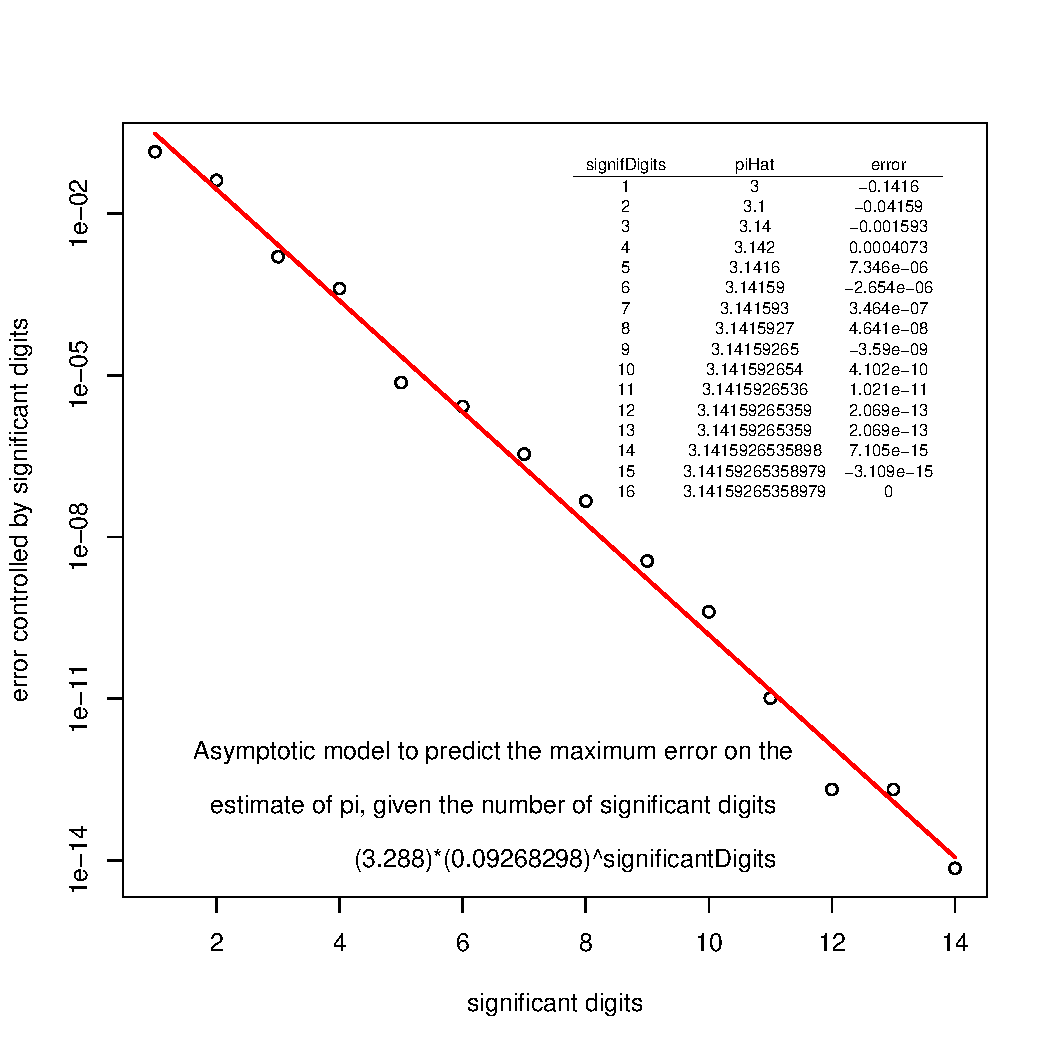
\includegraphics[scale=0.5]{fg_asym_pi_digits.pdf}
        \caption{This plot shows the error decreases as the
        significant digits increase in the experiement}
    \end{center}  
    \end{figure} 
     
    \begin{figure}[H]
        \begin{center}
            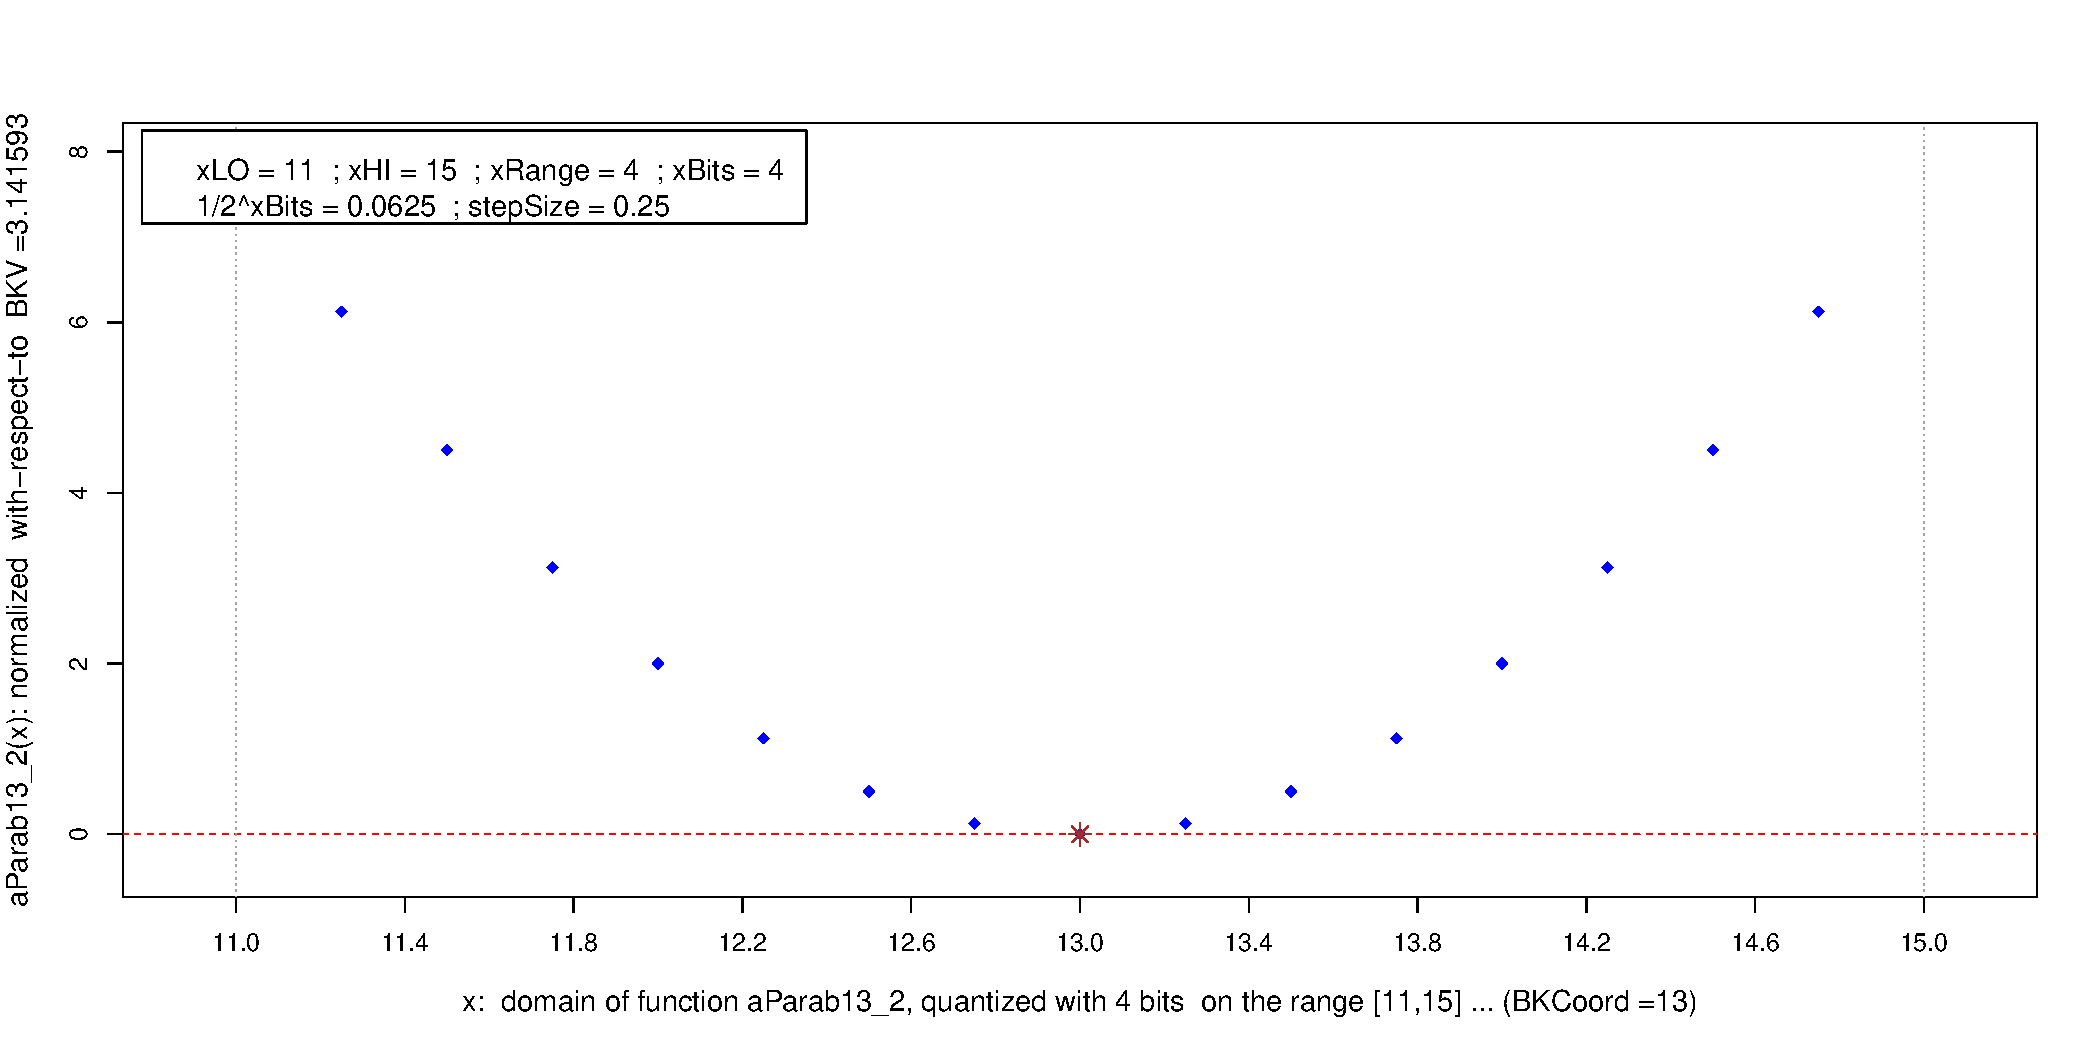
\includegraphics[scale=0.4]{fg_OF_aParab13_2_quant_exh.pdf}
            \caption{This plot is the aparab13 function}
        \end{center}
    \end{figure}

    \begin{figure}[H]
        \begin{center}
            \includegraphics[scale=0.5]{}
        \end{center}
    \end{figure}
    

\end{document}